\documentclass[a4paper,notitlepage,twoside]{book}
\usepackage{graphicx,subfigure}
\usepackage{abc}
\usepackage{verbatim}
\usepackage{pdfpages}
\usepackage{etoolbox}
\usepackage{wrapfig}
\usepackage{etoolbox}
\usepackage{setspace}
\AtBeginEnvironment{quote}{\singlespace\vspace{-\topsep}\small}
\AtEndEnvironment{quote}{\vspace{-\topsep}\endsinglespace}
            
\usepackage{makeidx}
\makeindex
\setlength{\parindent}{0em}
\setlength{\parskip}{1em}
\raggedbottom
\makeatletter
\let \@sverbatim \@verbatim
\def \@verbatim {\@sverbatim \verbatimplus}
{\catcode`'=13 \gdef \verbatimplus{\catcode`'=13 \chardef '=13 }} 
\patchcmd{\verbatim@input}{\@verbatim}{\footnotesize\@verbatim}{}{}
\makeatother
 
\usepackage[a4paper, total={20cm, 28cm},margin=1in]{geometry}
%\pagenumbering{gobble}
\usepackage{hyperref}
\hypersetup{
    colorlinks=true, %set true if you want colored links
    linktoc=all,     %set to all if you want both sections and subsections linked
    linkcolor=blue,  %choose some color if you want links to stand out
}

\title{
{\em The Society for the Preservation and Promotion \\of Machine Folk Music (v1.1)} \\
\begin{center}
\includegraphics[width=\textwidth]{front2.png}
\end{center}
\vspace{0.5in}The {\em Official} Tunebook \\
with Interesting Information about a Fascinating Hobby
\vfill
\small
The Society for the Preservation and Promotion of Machine Folk Music (v1.1)
was established in 2020, with support of the project,
{\em Music at the Frontiers of Artificial Creativity and Criticism (MUSAiC)}
(European Research Council Consolidator grant ERC-2019-COG, No. 864189),
Bob L. T. Sturm presiding.
}
%\date{}
%\author{folk-rnn}

\begin{document}
\frontmatter
\maketitle

\chapter{Praise for Machine Folk and The Society}
\begin{itemize}
\item ``I like to think that music comes from somewhere that’s living. Otherwise it’s…something else. Algorithms, computers - they’ll always be predictable. Not so much humans. ... My concern is that some people, somewhere and sometime, may consider one or more of these tunes - maybe all of them? - to be actual traditional tunes.'' \href{https://thesession.org/discussions/39604}{{\em Ergo}}
\item ``The most useless piece of shit ever. Fuck off with that crap.'' \href{https://consequenceofsound.net/2017/05/meet-bot-dylan-the-ai-computer-that-can-write-its-own-folk-songs/}{{\em fuckthat}}
\item ``I don’t know whether to applaud or cry.'' \href{https://thesession.org/discussions/42712}{{\em John K.}}
\item ``Machines aren't creative as this proves.'' \href{https://www.breitbart.com/tech/2017/05/26/bot-dylan-computer-composer-creates-100000-new-folk-songs/}{{\em tz1}}
\item ``Why. Machine art is not human therefore just a soulless imitation. If it imitates it cannot create anything new.'' \href{https://www.dailymail.co.uk/sciencetech/article-4544400/Researchers-create-computer-writes-folk-music.html#comments}{{\em worddust, Woodbridge}}
\item ``Totally lifeless without warmth. Mind you much human tuneless junk that passes for music today isn't much better.'' \href{https://www.dailymail.co.uk/sciencetech/article-4544400/Researchers-create-computer-writes-folk-music.html#comments}{{\em Mikeyt1941, London}}
\item ``Isn't music robotic enough these days?'' \href{https://www.dailymail.co.uk/sciencetech/article-4544400/Researchers-create-computer-writes-folk-music.html#comments}{{\em rocksnoop1, Dover}}
\item ``Basically it’s crude turntabling without the sense of a musician familiar with the significance of various motifs \& phrases.'' \href{https://thesession.org/discussions/37800}{{\em AB}}
\item ``Jeez. A computer that noodles. That’s all we need.'' \href{https://thesession.org/discussions/37800}{{\em Mark M.}}
\item ``This sounds like evil devil work.'' \href{https://thesession.org/discussions/37800}{{\em Jerone, LoM}}
\item ``Snacka om själ-lösa låtar... MUSIK.. Speciellt folkmusik.. Ska komma fram via upplevelser, traditioners djupa prägling. Upplevelser osv. Där människan är fokus, där folkmusiken präglat det traditionella kulturella livet. ... När jag ser sådant här blir jag antingen förbannad eller skitskarp. \href{https://www.facebook.com/groups/svenskfolkmusik/permalink/10156536106241145/}{{\em Stefan J.}}
\item ``Let's make all humans redundant, brilliant! Has everybody really lost their soul?!'' \href{https://www.dailymail.co.uk/sciencetech/article-4544400/Researchers-create-computer-writes-folk-music.html#comments}{{\em pen, somewhere}}
\item ``This takes away possibilities for real musicians to compose Music and earn a living!'' \href{https://www.facebook.com/groups/svenskfolkmusik/permalink/10156536106241145/}{{\em Per S.}}
\item ``Correct me if I'm wrong, but isn't music supposed to come from the soul. Isn't it an expression of our humanity aren't the sentiments expressed supposed to touch us and make us empathise with the song writer/singer. AI generated music does none of those things, therefore it's pointless. It's like comparing a machine made chair to a Chippendale. Yes you can sit on both of them, but the beauty of a handmade, beautifully crafted chair cannot be compared to a mass produced conveyor belt item.'' \href{https://www.dailymail.co.uk/sciencetech/article-4544400/Researchers-create-computer-writes-folk-music.html#comments}{{\em babsg, Newcastle}}
\item ``I think there is still some hope for humankind... Truthfully, if I learnt a tune by mistake that was written by a computer I would drop it. There are too many great tunes with a human story. A tune named ``Johnny O’Leary’s" will have at least some connection - how it got from there to here through people. A tune called ``Macbook Pro’s" just doesn’t have the same allure.'' \href{https://thesession.org/discussions/42458}{{\em bogman}}
\item ``This computerized AI is just so non musically untalented lazy nerds can infiltrate the world of true musicians who love, created, and write the music from the joy, hurt, and life emanating from their hearts.'' \href{https://www.dailymail.co.uk/sciencetech/article-4544400/Researchers-create-computer-writes-folk-music.html#comments}{{\em Radar Also, Hemet}}
\item ``I would suggest confining your computerised efforts to the archives of whichever University you are at.'' \href{https://thesession.org/discussions/39604}{{\em anonymous}}
\item ``Can we not technologically tamper with everything that is good and pure in this world? A computer farting out generated tunes in some academic lab somewhere is the beginning of the end. ... The sooner this experiment is confined to an anonymous university archive the better.'' \href{https://thesession.org/discussions/40416}{{\em anonymous}}
\item ``It’s a niche interest within a niche interest that will go under the radar of all but those most interested in the area and won’t have the slightest effect on the lives of the vast majority of us. It’s probably less useful in practical terms than building algorithms to direct robot vacuum cleaners or self-driving cars, but why knock it as a field of study? Most career academics that I know are deeply buried in some very esoteric trench in their field.'' \href{https://thesession.org/discussions/39604}{{\em Namloc}}
\item ``There are loads of crap tunes written by humans and there will continue to be (as long as there are people like me) in perpetuity. I’d rather play a great tune written by a computer than a crap one I wrote myself.'' \href{https://thesession.org/discussions/39604}{{\em Conán M.}}
\end{itemize}

\tableofcontents
\mainmatter
\chapter{Introduction}
This growing curated collection contains tunes
arising from creative partnerships with {\em music Ai}. %\footnote{``Ai'' is an acronym for ``artificial intelligence''. 
%We do not capitalize the ``i'' because the ``intelligence'' is questionable.} 
Some Ai are trained on over 23,000 music transcriptions 
contributed by users of \href{http://thesession.org}{\tt thesession.org},
which is focused on Irish traditional dance music.
These are named {\em folk-rnn} v1, v2 and v3. 
The different versions arise from
different formats of the training material:
v1 models character sequences in a single document, 
including tune titles;
v2 models tokenized transcriptions that have been transposed to 
have a root of C;
v3 uses a slightly different data representation from v2.
Another Ai, {\em folk-rnn} (v. Swedish), was tuned using 4,000 transcriptions of 
Scandinavian folk music, collected from \href{http://folkwiki.se}{\tt folkwiki.se}.
Other variants of these systems have also been produced,
e.g., using different sampling techniques.

Each transcription herein revealed itself to the world 
through a computational procedure involving on average one billion operations.
They are not purely products of a cold and lifeless statistical algorithm 
attempting to imitate patterns it has learned from existing data ---
some human operator is needed to ``flip the switch'',
and then to curate from the materials generated.
Often the Ai generates poor results. 
Sometimes they are clearly derivative.
In a few cases, they can be unusual and wonderful.
The challenge is to find these ``diamonds'' in the raw materials.
%How easy is it to find these gems that are worth the time learning?
Then to bring them to life without ever heard them
played before by a master musician.
%How easily can a transcription be interpreted using 
%the ``templates'' of, say, Irish traditional music?
Even so, there remains the problem
of a tune existing without any trace whatsoever 
in a collective memory of a community of practitioners.
Their context is digital vapor.

Some believe in a purity or divinity of Art, and the superiority of humans in making Art. 
Involving a machine in Art can be seen as a direct challenge to this purity, 
not to mention a demotion of the human to machine. 
This argument elevates the tangible product over the intangible experience, 
and submits to a rather narrow and mystical notion of creating Art ---
a human activity, full stop. It is an activity that occurs between our ears in our sensations, thoughts and memories. Art is not contained on the page or in the frame. It does not stop when we leave the concert hall or the museum. Art is entirely steeped in being human. The human decision to involve technology in that activity is only that: the suspension of pigment in egg yolk to make it stick to a surface; the suspension of pigment in slow-drying oil to make it blend and layer in ways superior to egg tempura; the suspension of pigment in plastic medium to make it sculptable and fast drying; the use of a coarse horse hair brush to paint several strands of hair at once; the use of a palette knife to make sharp straight edges; the use of the principles of geometry and perspective to create trompe-l'œil. How is involving Ai in creating music any different? 
Computers have been able to beat the best human chess players for decades, 
but for some reason people are still playing and studying chess. Why?

One pitfall important to avoid when it comes to discussing Ai in the Arts is this: 
thinking that the terms “intelligence” and “learning” mean what they commonly mean when it comes to people. These are “suitcase” words with several meanings that can be confused, and must be unpacked. In the context of Ai, “intelligence” is a quite brittle thing that bears very little resemblance to human intelligence. And “learning” is merely the prosaic computation of numbers in an algorithm that represent probabilistic relationships in data. Falling into this trap can give power to the Ai that it does not actually possess,
leading to dystopian fantasies.
To claim Ai will destroy music is the same as claiming, e.g., photography will destroy painting, perspective drawing will destroy narrative, and so on. Yes, the future is filled with composers and painters, photographers and writers … The only real threats to the Arts are the lack of value for it in a society, and proscriptions of practice due to pressures economic, political, religious, etc.


% Maybe someone has said, \href{https://www.bbc.com/news/technology-50573071}{“Why should I continue playing if I can never beat the computer?”} I would then wonder why they put so much weight on winning that it precludes them from playing? I bring up chess playing because when I compose or learn a tune, I think of it as an enjoyable intellectual challenge, much like playing chess. The experience is the most important part for me, not necessarily the end result.

\section{Inspirations}
\begin{enumerate}
\item \href{https://www.soundohm.com/product/the-last-lp}{Michael Snow, ``The Last LP: Unique Last Recordings Of The Music Of Ancient Cultures''}
\item Jennifer Walshe's \href{http://www.aisteach.org/}{The Avant Garde Archive of Ireland ({\tt aisteach.org})}
\item \href{http://milker.org/ghosts-of-the-hidden-layer}{Jennifer Walshe, ``Ghosts of the Hidden Layer''
seminar at Darmstädter Ferienkurse, July 25 2018}
\item \href{http://www.dramonline.org/labels/league-of-automatic-music-composers}{League of Automatic Music Composers}
\item Hobsbawm and Ranger (eds), ``The Invention of Tradition'', Cambridge University Press, 2012.
\end{enumerate}
\section{Key References}
\begin{enumerate}
\item \href{https://www.facebook.com/groups/TheMFSociety/}{The Society for the Preservation and Promotion of Machine Folk Music (v1.1) facebook group}
\item \href{https://github.com/boblsturm/MFSocietyTunebook}{Tunebook repository}
%\item \href{https://drive.google.com/open?id=1XgGBxKvZStMrwhMwqtsEFLH8owAnEpcW}{The Google Drive of The Society}
\item \href{https://folkrnn.org/}{{\tt folkrnn.org}}
\item \href{https://themachinefolksession.org/}{{\tt themachinefolksession.org}}
\item \href{https://github.com/IraKorshunova/folk-rnn}{The computer code and data behind folk-rnn}
\item \href{https://highnoongmt.wordpress.com/2018/01/05/volumes-1-20-of-folk-rnn-v1-transcriptions}{The folk-rnn Session Books (34 volumes of 100,000 transcriptions)}
\item \href{https://soundcloud.com/oconaillfamilyandfriends}{``Let's Have Another Gan Ainm'': An experimental album of Irish traditional music and computer-generated tunes} (\href{http://urn.kb.se/resolve?urn=urn:nbn:se:kth:diva-235167}{Technical Report})
\item Sturm et al., ``\href{https://arxiv.org/pdf/1604.08723}{Music transcription modelling and composition using deep learning}", in Proc. 1st Conf. Computer Simulation of Musical Creativity, July 2016.
\item Sturm and Ben-Tal, ``\href{https://www.jcms.org.uk/article/id/517/}{Taking the Models back to Music Practice: Evaluating Generative Transcription Models built using Deep Learning},” J. Creative Music Systems 2(1) Sep. 2017.
\item Sturm, ``\href{http://urn.kb.se/resolve?urn=urn:nbn:se:kth:diva-238604}{What do these 5,599,881 parameters mean? An analysis of a specific LSTM music transcription model, starting with the 70,281 parameters of its softmax layer},” in Proc. Music Metacreation workshop of ICCC, 2018.
\item Sturm et al. ``\href{https://www.tandfonline.com/doi/full/10.1080/09298215.2018.1515233}{Machine learning research that matters for music creation: A case study},” J. New Music Research 48(1):36-55, 2018.
\item Holzapfel, Sturm, and Coeckelbergh, “\href{https://transactions.ismir.net/articles/10.5334/tismir.13/}{Ethical dimensions of music information retrieval technology},” Trans. Int. Soc. Music Information Retrieval 1(1):44--55, 2018.
\item Sturm et al., “\href{https://www.mdpi.com/2076-0752/8/3/115}{Artificial intelligence and music: Open questions of copyright law and engineering praxis},” MDPI Arts 8(3), 2019.
\item Hallstr\"om et al., ``From Jigs and Reels to Schottisar och Polskor: Generating Scandinavian-like Folk Music with Deep Recurrent Networks,'' in Proc. Sound \& Music Computing Conf., 2019.
\item Ben-Tal, Harris, and Sturm, ``\href{https://www.mitpressjournals.org/doi/abs/10.1162/leon_a_01959}{How music AI is useful: Engagements with composers, performers, and audiences},'' Leonardo Music Journal (2020).
\end{enumerate}

\section{Appearances of Members of The Society}
\begin{enumerate}
\item \href{https://www.facebook.com/events/121474282609573/}{Feb 26 2020} at the Austrian Research Institute for Artificial Intelligence, Vienna
\item \href{https://wasp-hs.org/events/kick-off-wasp-hs/}{Mar 12 2020} at ``AI for Humanity and Society 2020'', Stockholm (cancelled due to COVID-19, but rescheduled Nov. 18 2020)
\item \href{https://ars.electronica.art/keplersgardens/en/kth/}{Sep 11 2020} at Ars Electronica 2020
\item \href{https://boblsturm.github.io/aimusic2020/}{Oct 19 2020} at The 2020 Joint Conference on AI Music Creativity 
\item \href{https://www.ebu.ch/events/2021/02/ai-for-content-creation}{Feb 9 2021} AI for Content Creation, European Broadcasting Union
\item \href{https://www.umu.se/en/events/music-ai-and-digital-tools_10320887}{Apr 23 2021} Umeå Humanities Lab
\item \href{https://aamas2021.soton.ac.uk/programme/social-activities}{May 6 2021} 20th International Conference on Autonomous Agents and Multiagent Systems
\end{enumerate}

\section{Frequently Asked Questions}
\begin{enumerate}
\item ``What is {\em machine folk}?''\\
Music that springs from human and machine (Ai) partnership,
played on traditional instruments as if such a thing has been done for centuries.
Other terms for this kind of music are: {\em faux folk} and {\em trAiditional music}. 
%\item ``How is {\em machine folk} different from {\em fake folk}?\\
%{\em Machine folk} becomes {\em fake folk} with fabricated folklore. (See present volume.)
\item ``Why {\em machine folk}?''\\
Why not?
\item ``I mean, why not play {\em real} traditional music?''\\
Let's!
\item ``Do we really need to involve Ai in music?''\\ 
No, in the same way that we don't really need to involve pianos. 
\item ``Why do you have a lower-case `i' when you write `Ai'''?\\
To highlight the fact that its ``intelligence'' is questionable.
\item ``Isn't music robotic enough these days?'' \\
%Depends what is meant by ``music''. 
%``Robotic'' is an aim for some styles, e.g., sequenced, electronic dance music.
%For {\em machine folk}, ``robotic'' need not be the aim,
%or an unavoidable outcome.
What's wrong with ``robotic''?
\item ``I mean, isn't music supposed to come from the soul? Isn't it an expression of our humanity? Aren't the sentiments expressed supposed to touch us and make us empathize with the composer?'' \\
Who says those things? %Music has been, is, and continues to be far broader than simply expressing sentiments.
%Many of us have sentiments for machines. 
%Besides, it seems somewhat normal to care for an algorithm that
%one has built and watched grow.
%Playing {\em machine folk} is not an exclusionary practice.
%Plus there is something in {\em machine folk} that speaks of 
%a people awash in computer technology, data harvesting, surveillance, automation ...
%{\em Machine folk} is in a real sense an expression of our humanity vis-\`a-vis the machine.
\item ``Have you lost your soul?'' \\
Not that we are aware of; or, maybe yes?
Let's ask the machine to generate a tune about it.
\item ``Can we not technologically tamper with everything that is good and pure in this world?'' \\
Technological tampering is how musical instruments are created.
%We are definitely partial to the romantic idea of returning to the way things were 
%before fire was discovered and all hell broke loose.
%But then we realize that most  wouldn't exist.
\item ``Are you working to replace human composers and musicians?'' \\
No. Humans are an essential part of {\em machine folk},
from the programming and training of the Ai, 
to the curation of the generated music and its performance in the real world
on real instruments.
\item ``Won't this technology lead to replacing human composers and musicians?'' \\
If something can be automated, it will be automated.
Regardless if an Ai can compose music,
humans will continue to compose.
%Suffering is an essential part of the human condition.
\item ``Who owns these tunes?'' \\
The meaningfulness of this question is not clear in a society that has decided it's acceptable to not pay for music.\footnote{Compliments to \href{https://www.thefader.com/2020/02/25/holly-herndon-ai-generated-travis-scott-song-travisbott-jack-park-canny-dope-man-interview}{Holly Herndon}.}
Regardless, traditional music sits uncomfortably with such notions because it is much more like a public park for all to enjoy than private property for one to rent. The output of folk-rnn might be considered more like the public park – perhaps a little derelict with some broken glass and rusty nails laying around. No place for a picnic really; but still, many of its nooks and crannies are wonderful to visit and explore.
\item ``How will this help traditional music?''\\
Does traditional music need help?
%We are more concerned with how this could harm traditional music.
\item ``OK. How will this harm traditional music?''\\
Likely not one bit. These machines are just parlour tricks.
But it is important to keep watch for unintended consequences.
%\item ``By what criteria does The Society select tunes for this tunebook?''\\
%The criteria have yet to be formally defined,
%but certainly among them are things like musical sense, quirkiness, playability, and humor.
\end{enumerate}


\chapter{Tunes of the Society}
This chapter presents the tunes of the Society
categorized by rhythm.
When a tune involves some modification from 
the transcription produced by the machine, the original
is rendered as small notation.

\section{Jig}
\phantomsection
\addcontentsline{toc}{subsection}{Aloe Vera's}
\index{Aloe Vera's}\index{Jig ! Aloe Vera's}\index{folk-rnn (v2) ! Jig: Aloe Vera's}
\hypertarget{jig:AloeVeras}{\abcinput{AloeVerasjig}}
\begin{wrapfigure}{l}{0.4\textwidth}
\vspace{-0.3in}
\includegraphics[width=0.4\textwidth]{AloeVera.jpg}
\end{wrapfigure}
When Society Member Näsström shared the photo at left with the Society,
Member Sturm decided to ask folk-rnn (v2) to compose a jig about it.
The output, seen in small notation, was then modified a bit by Sturm to create the jig.
More information about this particular transcription is \href{https://themachinefolksession.org/tune/902}{here.}
One of Sturm's Irish accordion teachers says this tune sounds like the kind of new jigs
created by contemporary Irish composers, e.g., 
Mícheál Ó Súilleabháin.
Daniel Näsström (flute) and Sturm ({\em Bosca Dubh}): \url{https://youtu.be/jVJEEc90sxo}

\clearpage
\phantomsection
\addcontentsline{toc}{subsection}{The Boys of Ballinaburre}
\index{Boys of Ballinaburre, The}\index{Jig ! Boys of Ballinaburre, The}\index{folk-rnn (v2) ! Jig: Boys of Ballinaburre, The}
\hypertarget{jig:BoysofBallinaburre}{\abcinput{BoysofBallinaburre}}
This tune was learned from folk-rnn (v2),
which generated it under a particular sampling regimen.
More information \href{https://highnoongmt.wordpress.com/2019/08/19/making-sense-of-the-folk-rnn-v2-model-part-11/}{here}.
The title was generated by folk-rnn (v1) for a different tune, 
but applied to this tune because Society Member Sturm thinks it fits.
%\href{https://youtu.be/V8eYj7y2xn4}{Listen to Henrik Norbeck's interpretation of the tune.}
There's a claim that the turn (B-part) resembles that of a traditional Irish tune named, ``The Thatched Cabin''.
That particular tune does not appear in the training data of this folk-rnn model.
One of Sturm's Irish accordion teachers says this tune sounds like an old jig, 
and is ready to be learned as is.
Sturm ({\em Bosca Dubh}): \url{https://youtu.be/qcOZZpfSM_E}

\phantomsection
\addcontentsline{toc}{subsection}{Gallagher's Favourite}
\index{Gallagher's Favourite}\index{Jig ! Gallagher's Favourite}\index{folk-rnn (v3) ! Jig: Gallagher's Favourite}
\hypertarget{jig:GallaghersFavourite}{\abcinput{GallaghersFavourite}}
This tune appears in the \href{https://highnoongmt.wordpress.com/2018/01/05/volumes-1-20-of-folk-rnn-v1-transcriptions}{folk-rnn (v3) Session Book, Vol. 3 of 4} (\#5712).
The title was generated by folk-rnn (v1) for a different tune, 
but applied to this tune because Society Member Sturm thinks it fits.
Only one slight change is made to the last measure.
One of Sturm's Irish accordion teachers says
this sounds like a classic jig.
Sturm ({\em Bosca Dubh}): \url{https://youtu.be/y6-7bLIJS9g}

\phantomsection
\addcontentsline{toc}{subsection}{Cleaper's Wheel}
\index{Cleaper's Wheel}\index{Jig ! Cleaper's Wheel}\index{folk-rnn (v2) ! Jig: Cleaper's Wheel}
\hypertarget{jig:CleapersWheel}{\abcinput{CleapersWheel}}
The Society members Larsson, Kmoch and Sturm found this tune together 
while browsing the \href{http://www.eecs.qmul.ac.uk/~sturm/research/RNNIrishTrad/Session/}{Endless MF Session website}
(\href{http://www.eecs.qmul.ac.uk/~sturm/research/RNNIrishTrad/Session/5583_11843.mp3}{synthesized recording}).
The title was generated by folk-rnn (v1) for a different tune, 
but applied to this tune because Society Member Sturm thinks it fits.
It appears in the \href{https://highnoongmt.wordpress.com/2018/01/05/volumes-1-20-of-folk-rnn-v1-transcriptions}{folk-rnn (v2) Session Book, Vol. 2 of 10}.
One of Sturm's Irish accordion teachers pointed out that
the first part of the tune closely resembles the jig ``Old Man Dillon'',
but the second part is completely unique and wonderful.
Society Member Sturm thus modified the first part.

\phantomsection
\addcontentsline{toc}{subsection}{The A.i. Man}
\index{A.i. Man, The} \index{Jig ! A.i. Man, The} \index{folk-rnn (v2) ! Jig: A.i. Man, The}
\hypertarget{jig:Aiman}{\abcinput{AIMan}}
This jig won the first place prize at the 
\href{https://highnoongmt.wordpress.com/2020/11/20/the-ai-music-generation-challenge-2020-summary-and-results/}{Ai Music Generation Challenge 2020}.
The title was given to it by judge Paudie O'Connor.
The jig was generated by folk-rnn (v2), sampled with beamsearch (n=2),
and selected by an artificial critic comparing the outputs
with O'Neill's 365 double jigs in the ``1001'' collection.
In the 10001 jigs generated by the system and selected by the critic,
it appears as \#8091.
Sturm ({\em Bosca Dubh}): \url{https://youtu.be/yhPuYbhr7Y4}
  
\phantomsection
\addcontentsline{toc}{subsection}{Wolden Sailor}
\index{Wolden Sailor} \index{Jig ! Wolden Sailor} \index{folk-rnn (v2) ! Jig: Wolden Sailor}
\hypertarget{jig:WoldenSailor}{\abcinput{WoldenSailor}}
This tune appears in the \href{https://highnoongmt.wordpress.com/2018/01/05/volumes-1-20-of-folk-rnn-v1-transcriptions}{folk-rnn (v2) Session Book, Vol. 7 of 10} (\#18727).
The title was generated by folk-rnn (v1) for a different tune, 
but applied to this tune because Society Member Sturm thinks it fits.
Sturm ({\em Bosca Dubh}): \url{https://youtu.be/t7yMv2B6MNQ}
  
\phantomsection
\addcontentsline{toc}{subsection}{The Rellus On The Turnpipe}
\index{Rellus On The Turnpipe, The} \index{Jig ! Rellus On The Turnpipe, The} \index{folk-rnn (v1) ! Jiog: Rellus On The Turnpipe, The}
\hypertarget{jig:RellusTurnpipe}{\abcinput{RellusTurnpipe}}
This delicate jig was generated by folk-rnn (v1), which also titled it.
It appears in the \href{https://highnoongmt.wordpress.com/2018/01/05/volumes-1-20-of-folk-rnn-v1-transcriptions}{folk-rnn (v1) Session Book, Vol. 8 of 20}.
Sturm ({\em Bosca Dubh}): \url{https://youtu.be/JrUa-RSpN78}

\phantomsection
\addcontentsline{toc}{subsection}{The Lonesome Fairy}
\index{Lonesome Fairy, The} \index{Jig ! Lonesome Fairy, The} \index{folk-rnn (v2) ! Jig: Lonesome Fairy, The}
\hypertarget{jig:LonesomeFairy}{\abcinput{LonesomeFairy}}
This jig won the second place prize at the 
\href{https://highnoongmt.wordpress.com/2020/11/20/the-ai-music-generation-challenge-2020-summary-and-results/}{AI Music Generation Challenge 2020}.
The title was given to it by judge Jennikel Andersson.
The jig was generated by folk-rnn (v2).
In the 10001 jigs generated by the system,
it appears as \#7983.
Sturm ({\em Bosca Dubh}): \url{https://youtu.be/FVIaI7VbV1A}

\phantomsection
\addcontentsline{toc}{subsection}{The Waters of Heanny}  
\index{Waters of Heanny, The} \index{Jig ! Waters of Heanny, The} \index{folk-rnn (v1) ! Jig: Waters of Heanny, The}
\hypertarget{jig:WatersofHeanny}{\abcinput{WatersofHeanny}}
This tune and its title appears in the \href{https://highnoongmt.wordpress.com/2018/01/05/volumes-1-20-of-folk-rnn-v1-transcriptions}{folk-rnn (v1) Session Book, Vol. 3 of 20}.
Society Member Sturm changed a few parts to make it more ``watery.''
The original output of the algorithm is shown in smaller notation.
Sturm ({\em Bosca Dubh}): \url{https://youtu.be/QehkSmrOJ_4}

\phantomsection
\addcontentsline{toc}{subsection}{My Ove Wore A Da'}  
\index{My Ove Wore A Da'} \index{Jig ! My Ove Wore A Da'} \index{folk-rnn (v2) ! Jig: My Ove Wore A Da'}
\hypertarget{jig:MyOve}{\abcinput{MyOve}}
This tune was learned from folk-rnn (v2) with beamsearch (n=2).
In the 10001 jigs generated by the system and selected by the critic,
it appears as \#18. 
The title was applied to this tune by a system taught to title tunes.
Sturm's accordion teacher agrees that it's a nice melody,
and plays well as a single jig.
Sturm ({\em Bosca Dubh}): \url{https://youtu.be/SU2jPwHiDfk}

\phantomsection
\addcontentsline{toc}{subsection}{The Teelin Brood}  
\index{Teelin Brood, The} \index{Jig ! Teelin Brood, The}\index{folk-rnn (v2) ! Jig: Teelin Brood, The}
\hypertarget{jig:TeelinBrood}{\abcinput{TeelinBrood}}
This jig generated by folk-rnn (v2) was selected by an artificial critic 
tuned to the likes of Society Member Sturm --- the same critic that suggested
the hornpipe ``Fredrik's Christmas Critic'' on page \pageref{tune:FredriksChristmasCritic}.
The title was generated by folk-rnn (v1) for a different tune
but Society Member Sturm believes it fits this one too.
Sturm ({\em Bosca Dubh}): \url{https://youtu.be/q6g9mX0IU2I}

\phantomsection
\addcontentsline{toc}{subsection}{Happy to Jeer}  
\index{Happy to Jeer} \index{Jig ! Happy to Jeer} \index{folk-rnn (v2) ! Jig: Happy to Jeer}
\hypertarget{jig:Happytojeer}{\abcinput{Happytojeer}}
This jig, generated by folk-rnn (v2),
was highly rated at the \href{https://highnoongmt.wordpress.com/2020/11/20/the-ai-music-generation-challenge-2020-summary-and-results/}{AI Music Generation Challenge 2020},
but did not win a prize. 
The title was applied to this tune by another system taught to title tunes.
In the 10001 jigs generated by the system and selected by the critic,
it appears as \#6021.
Sturm's Irish accordion teacher says it sounds like a classic jig 
used for teaching dancing.
Sturm ({\em Bosca Dubh}), Carla Sturm \& Shoogee: \url{https://youtu.be/FVacJEMReRA}

\phantomsection
\addcontentsline{toc}{subsection}{Garrett Farmor's}  
\index{Garrett Farmor's}\index{Jig ! Garrett Farmor's}\index{folk-rnn (v2) ! Jig: Garrett Farmor's}
\hypertarget{jig:GarrettFarmors}{\abcinput{GarrettFarmors}}
This tune was learned from folk-rnn (v2),
and appears as \#2857 in
the \href{https://highnoongmt.wordpress.com/2018/01/05/volumes-1-20-of-folk-rnn-v1-transcriptions}{folk-rnn (v2) Session Book, Vol. 1 of 10}.
More information on this tune can be found \href{https://highnoongmt.wordpress.com/2017/12/02/folk-rnn-v2-tune-2857/}{here.}
The title was generated by folk-rnn (v1) for a different tune, 
but applied to this tune because Society Member Sturm thinks it fits.
One of Sturm's Irish accordion teachers says this tune is {\em not} good -- actually, ``it's not even music'' --
which motivates Sturm to play it often because he strongly believes otherwise.
Sturm ({\em Bosca Dubh}): \url{https://youtu.be/4ldA8ub35-g}

\clearpage
\section{Reel}
\phantomsection
\addcontentsline{toc}{subsection}{Aloe Vera's}  
\index{Aloe Vera's}\index{Reel ! Aloe Vera's}\index{folk-rnn (v2) ! Reel:  Aloe Vera's}
\hypertarget{reel:AloeVeras}{\abcinput{AloeVerasReel}}
\begin{wrapfigure}{l}{0.4\textwidth}
\vspace{-0.3in}
\includegraphics[width=0.4\textwidth]{AloeVera2.jpg}
\end{wrapfigure}
The basic idea of this reel were generated by folk-rnn (v2) 
seeded with {\tt dcAB GABG} (but transposed to C major), 
which are the first eight pitches of \hyperlink{jig:AloeVeras}{Aloe Vera's} (jig).
The impetus of the tune came when Society Member Näsström shared the photo at left with the Society,
saying, ``Mother Aloe Vera just told me she want a reel.''
Sturm ({\em Bosca Dubh}): \url{https://youtu.be/Xb8RC6GgpLM}

\clearpage
\phantomsection
\addcontentsline{toc}{subsection}{Swing Swang Swung}  
\index{Swing Swang Swung}\index{Reel ! Swing Swang Swung}\index{folk-rnn (v2) ! Reel: Swing Swang Swung}
\hypertarget{reel:SwingSwangSwung}{\abcinput{SwingSwangSwung}}
This tune was learned from folk-rnn (v2).
The opening bears some similarity to ``Swing Swang'' 
\href{https://youtu.be/Fl3e4010epE?t=50}{played by Na Dra\'iod\'oir\'i}
(a tune that is in the training data of this model) ---
thus inspiring the title.
More information about this particular transcription is \href{https://highnoongmt.wordpress.com/2018/01/03/making-sense-of-the-folk-rnn-v2-model-part-5/}{here.}
One of Sturm's Irish accordion teachers says this is a good tune, and sounds like the kind of tunes he likes.
Sturm ({\em Bosca Dubh}): \url{https://youtu.be/1YOdeGgB_WY}

\phantomsection
\addcontentsline{toc}{subsection}{Roaring Sillow}  
\index{Roaring Sillow} \index{Reel ! Roaring Sillow} \index{folk-rnn (v2) ! Reel: Roaring Sillow} 
\hypertarget{reel:RoaringSillow}{\abcinput{RoaringSillow}}
This tune was created using folk-rnn v2 with beamsearch (n=4). It appears in the book chapter,
Sturm and Ben-Tal (2021). Handbook of Artificial Intelligence for Music, chapter Folk the Algorithms: (Mis)Applying Artificial Intelligence to Folk Music. Springer. 
The title was generated by folk-rnn (v1) for a different tune, 
but applied to this tune because Society Member Sturm thinks it fits.
Sturm ({\em Bosca Dubh}): \url{https://youtu.be/dNIIRhs-rhA}

\phantomsection
\addcontentsline{toc}{subsection}{Mickey Fitternaly’s}  
\index{Mickey Fitternaly’s}\index{Reel ! Mickey Fitternaly’s}\index{folk-rnn (v2) ! Reel: Mickey Fitternaly’s}
\hypertarget{reel:MickeyFitternalys}{\abcinput{MickeyFitternalys}}
This reel was learned from folk-rnn (v2),
which generated it under a particular sampling regimen.
The title was generated by folk-rnn (v1) for a different tune, 
but applied to this tune because Society Member Sturm thinks it fits.
More information \href{https://highnoongmt.wordpress.com/2019/08/19/making-sense-of-the-folk-rnn-v2-model-part-11/}{here}.
Society Member Sturm has slightly modified the last half of the sixth bar of the turn 
such that it repeats the 2nd bar of the turn. 
One of Sturm's Irish accordion teachers says this sounds like the kind of tunes he likes.
Sturm ({\em Bosca Dubh}): \url{https://youtu.be/Ewsvk6fy9Yg}

\phantomsection
\addcontentsline{toc}{subsection}{Close Encounters of the Reel Kind}  
\index{Close Encounters of the Reel Kind}\index{Reel ! Close Encounters of the Reel Kind}\index{folk-rnn (v2) ! Reel: Close Encounters of the Reel Kind}
\hypertarget{reel:CloseEncountersReel}{\abcinput{CloseEncountersReel}}
This tune was co-created with folk-rnn (v2).
The system was primed with {\tt M:4/4 K:Cmaj d e c C G 2},
which is the famous musical message to the extraterrestrials in 
the movie ``Close Encounters of the Third Kind.''
Proper performance of this tune dictates that the musicians look skyward for any ``signs''.
Sturm ({\em Bosca Dubh}): \url{https://youtu.be/ZN0Fi_oyu44}
  
\phantomsection
\addcontentsline{toc}{subsection}{The dog ate a raisin so call the vet}  
\index{The dog ate a raisin so call the vet} \index{Reel ! The dog ate a raisin so call the vet} \index{folk-rnn (v2) ! Reel: The dog ate a raisin so call the vet}
\hypertarget{reel:DogRaisin}{\abcinput{DogRaisin}}
\begin{wrapfigure}{l}{0.4\textwidth}
\vspace{-0.3in}
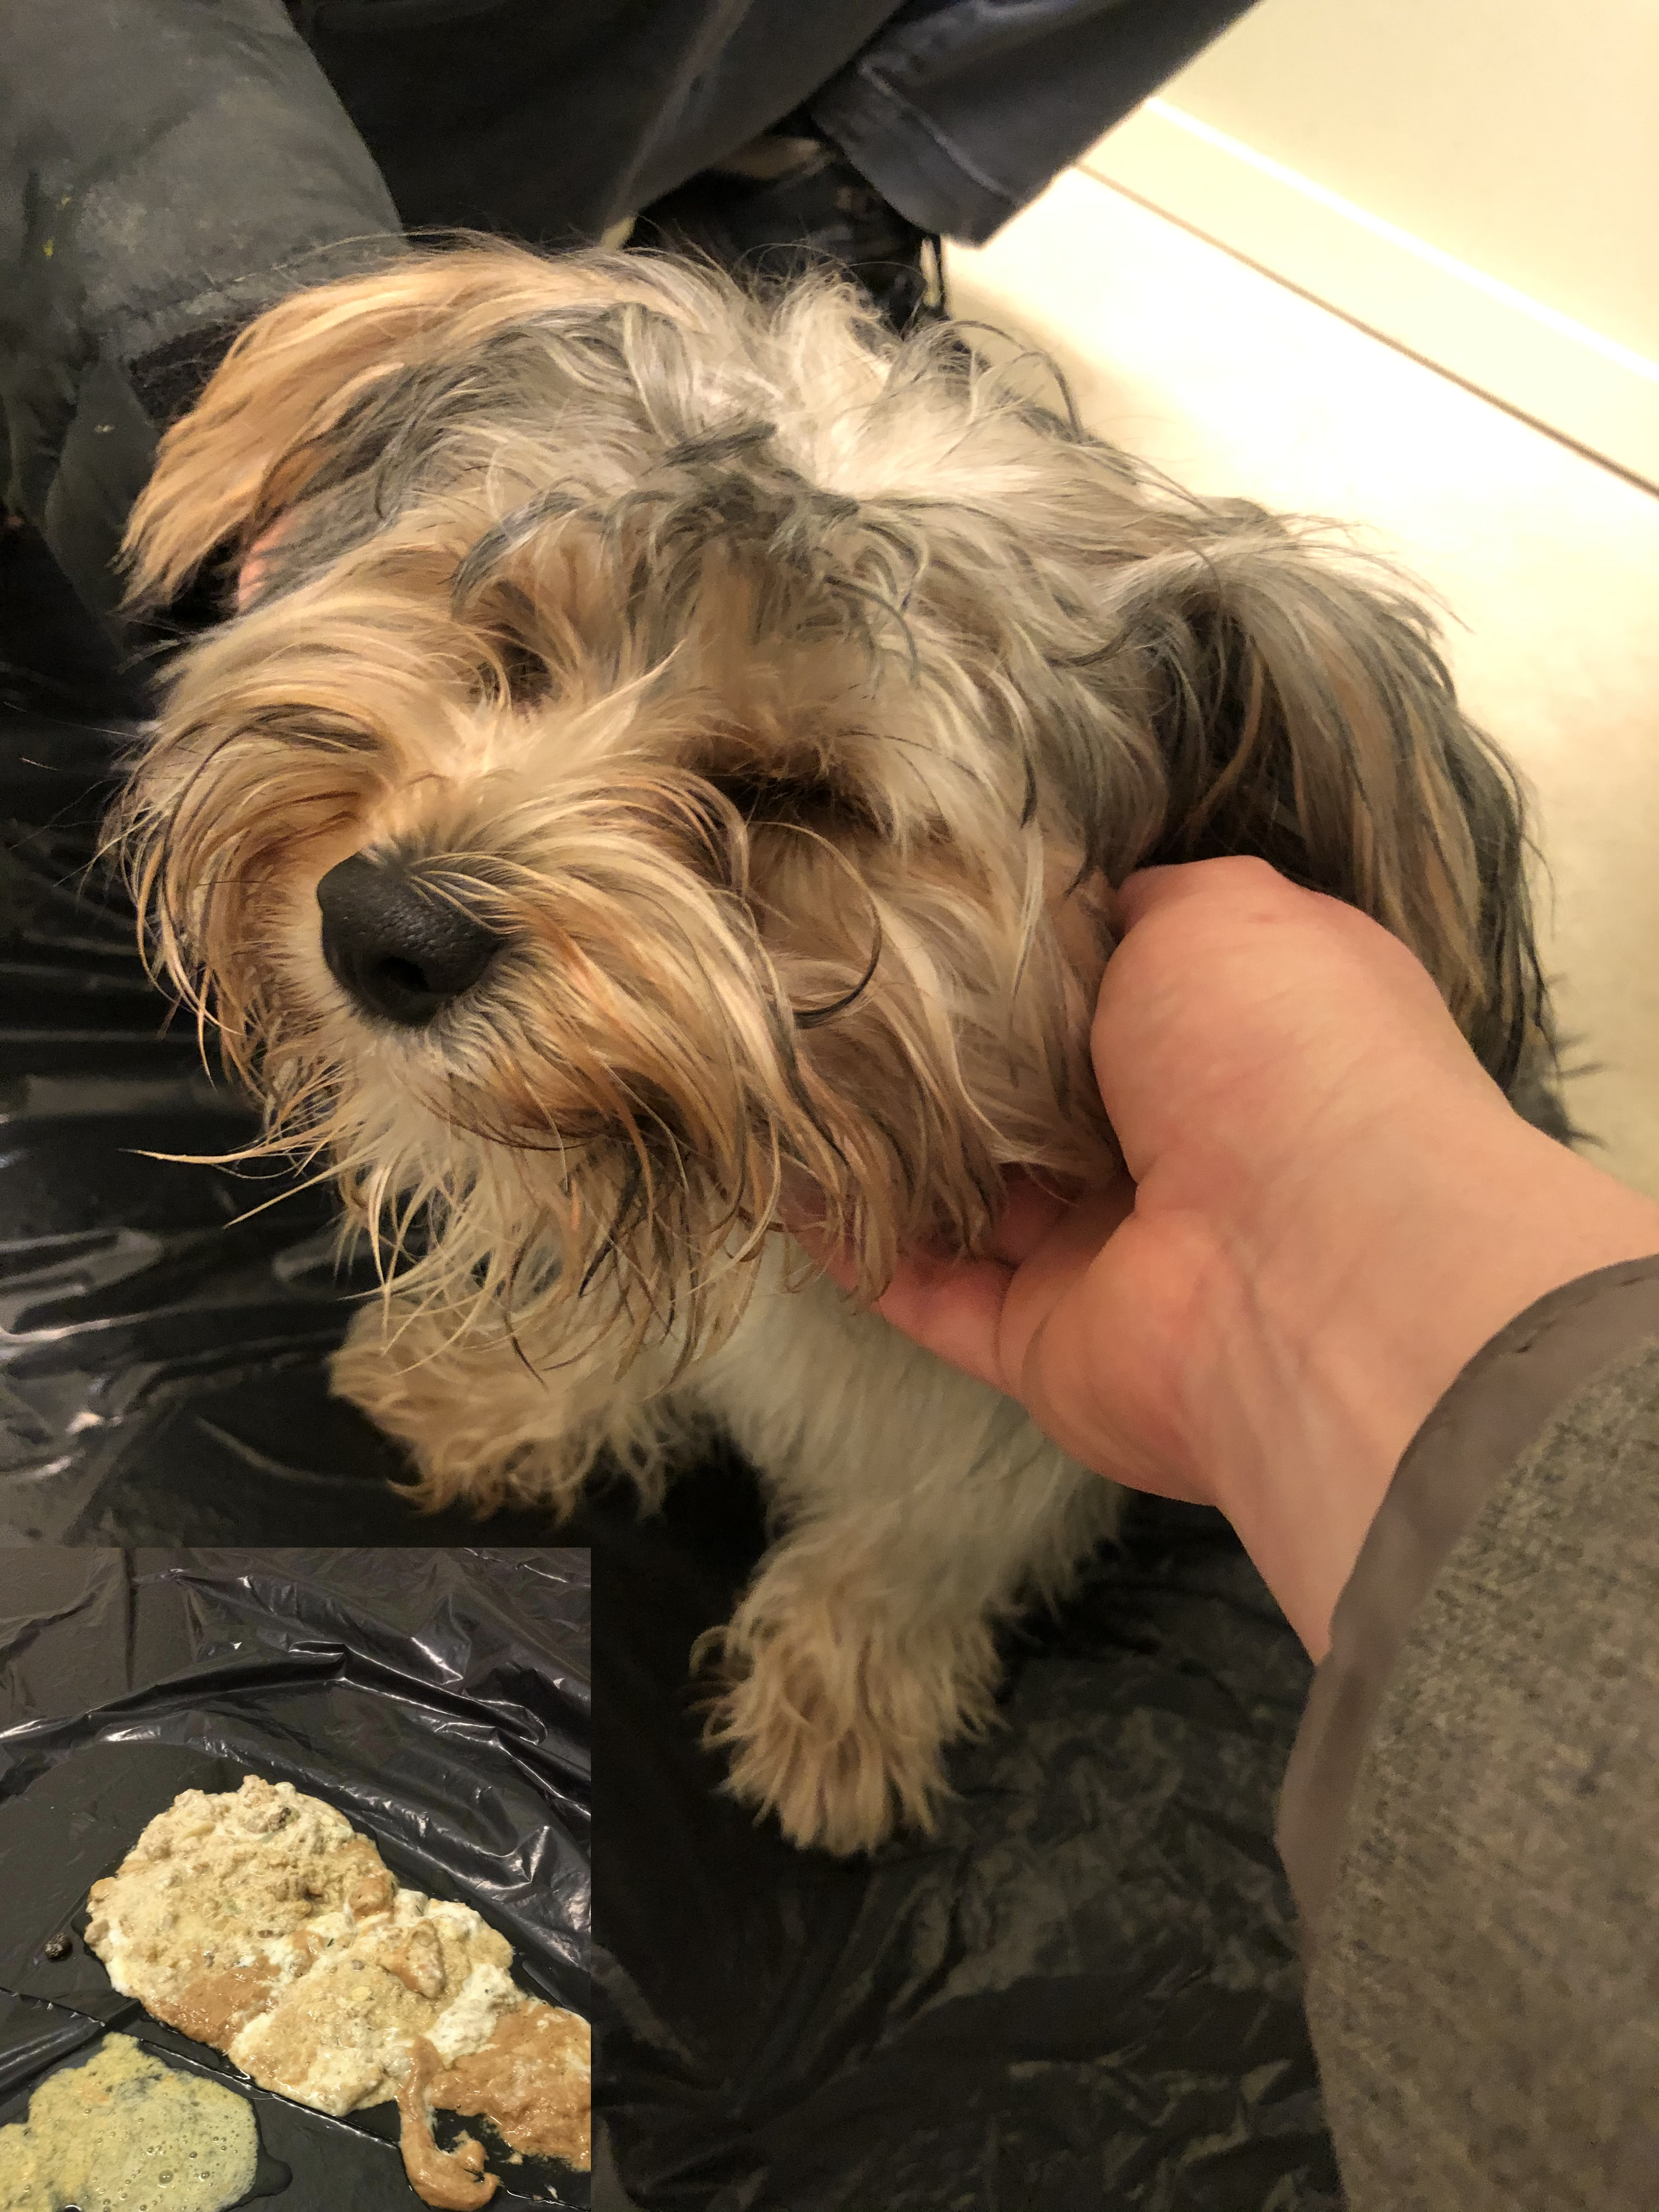
\includegraphics[width=0.4\textwidth]{ShoogeeVet.png}
\end{wrapfigure}
This reel generated by folk-rnn (v2) was selected by an artificial critic 
tuned to the likes of Society Member Sturm.
The title refers to Sturm's dog Shoogee,
who one morning ate a raisin, 
precipitating a quick visit to the vet
whereupon said raisin was ``extracted'' (inset of pictured).
Sturm ({\em Bosca Dubh}): \url{https://youtu.be/1PbTqFVAY64}

\clearpage
\phantomsection
\addcontentsline{toc}{subsection}{Shoogee Take Another Shoe}  
\index{Shoogee Take Another Shoe} \index{Reel ! Shoogee Take Another Shoe} \index{folk-rnn (v2) ! Reel: Shoogee Take Another Shoe}
\hypertarget{reel:ShoogeeTakeAnotherShoe}{\abcinput{ShoogeeTakeAnotherShoe}}
This reel generated by folk-rnn (v2) was selected by ``Fredrik's critic'' 
tuned to the likes of Society Member Sturm.
The title refers to Sturm's dog Shoogee,
who likes to run off with shoes. 
Sturm ({\em Bosca Dubh}): \url{https://youtu.be/ICN17681QwM}

\clearpage
\section{Hornpipe}
\phantomsection
\addcontentsline{toc}{subsection}{Ms. Riddles' Hornpipe}  
\index{Ms. Riddles' Hornpipe}\index{Hornpipe ! Ms. Riddles' Hornpipe} \index{folk-rnn (v2) ! Hornpipe: Ms. Riddles' Hornpipe}
\hypertarget{hornpipe:MsRiddles}{\abcinput{MsRiddles}}
\begin{wrapfigure}{l}{0.7\textwidth}
\includegraphics[width=0.4\textwidth]{MsRiddles.png}
\includegraphics[width=0.3\textwidth]{MsRiddles2.png}
\end{wrapfigure}
Society member Sturm got this hornpipe from folk-rnn (v2) 
when he asked it for a tune about the spider living in his bathroom – whom he named “Ms. Riddles”.
For one wonderful week, the silverfish in his bathroom disappeared thanks to Ms. Riddles. To show his gratitude, he caught and froze a fly, and gave it to Ms. Riddles. She seemed to enjoy eating it, and used it to decorate her porch, along with what appears to be the King of the Silverfish.
Ms. Riddles is long gone now, but her memory lives on in this wonderful hornpipe.
Sturm ({\em Bosca Dubh}): \url{https://youtu.be/V2EiFb89koE}

\phantomsection
\addcontentsline{toc}{subsection}{The Liddle Shepe}  
\index{Liddle Shepe, The}\index{Hornpipe ! Liddle Shepe, The}\index{folk-rnn (v2) ! Hornpipe: Liddle Shepe, The}
\hypertarget{hornpipe:LiddleShepe}{\abcinput{LiddleShepe}}
This lovely hornpipe was learned from folk-rnn (v2),
which generated it under a particular sampling regimen.
The title was generated by folk-rnn (v1) for a different tune, 
but applied to this tune because Society Member Sturm thinks it fits.
Society member Näsström says this tune makes him happy.
More information \href{https://highnoongmt.wordpress.com/2019/08/19/making-sense-of-the-folk-rnn-v2-model-part-11/}{here}.
One of Sturm's Irish accordion teachers says this tune is more like a strathspey or highland 
than a hornpipe --- the melody has phrases that sound too short for a hornpipe.
Sturm ({\em The Black Box}): \url{https://youtu.be/dvri_8zTXiI}
  
\phantomsection
\addcontentsline{toc}{subsection}{Fredrik's Christmas Critic}  
\index{Fredrik's Christmas Critic}\index{Hornpipe ! Fredrik's Christmas Critic}\index{folk-rnn (v2) ! Hornpipe: Fredrik's Christmas Critic}
\hypertarget{hornpipe:FredriksChristmasCritic}{\abcinput{FredriksChristmasCritic}}
This hornpipe was selected by an artificial critic choosing from tunes generated by folk-rnn (v2). The artificial critic was built by a student supervised by Society Member Sturm in the Fall 2020, named Fredrik. He sent  this tune as an example of a ``high scoring tune'', according to said critic. Sturm fell in love with it pretty quickly. More like this please, dear artificial critic! Sturm ({\em Bosca Dubh}): \url{https://youtu.be/Igwv5sgGlwU}

\phantomsection
\addcontentsline{toc}{subsection}{Sorpike’s Cat}  
\index{Sorpike’s Cat} \index{Hornpipe ! Sorpike’s Cat} \index{folk-rnn (v1) ! Hornpipe: Sorpike’s Cat}
\hypertarget{hornpipe:SorpikesCat}{\abcinput{SorpikesCat}}
This hornpipe was generated by folk-rnn (v1), and
appears in the \href{https://highnoongmt.wordpress.com/2018/01/05/volumes-1-20-of-folk-rnn-v1-transcriptions}{folk-rnn (v1) Session Book, Vol. 8 of 20}.
Sturm ({\em Bosca Dubh}): \url{https://youtu.be/uSPDnew-7sY}

\clearpage
\section{Polka}
\phantomsection
\addcontentsline{toc}{subsection}{Göran's sick at home and Pelle's just cut his finger}  
\index{Göran's sick at home and Pelle's just cut his finger} \index{Polka ! Göran's sick at home and Pelle's just cut his finger}\index{folk-rnn (v2) ! Polka: Göran's sick at home and Pelle's just cut his finger}
\hypertarget{polka:GoranPelle}{\abcinput{GoranPelle}}
This tune was co-created with folk-rnn (v2), seeding it with two ideas: 
one for the first part provided by Society member Sturm, 
and one for the second part provided by Society member Näsström. 
They wanted to write a polka for their two friends Göran and Pelle, 
with whom they play and enjoy Irish music. 
Göran couldn't make a session because he was sick, 
and Pelle had to cancel because he had cut his finger.
The system was seeded with {\tt |:c/2d/2e dc | BG B2} to create first part,
and then 
{\tt |:c/2d/2edc |BGB2 |c/2d/2e/2d/2cd |ed/2c/2BG | cd/2e/2dc |BGBB |c2B/2c/2d |c2c2 :| |:c'b gc' | bg}
to create second part.
Sturm ({\em Bosca Dubh}): \url{https://youtu.be/plZMHUDsmr0}

\phantomsection
\addcontentsline{toc}{subsection}{William Murphy's}  
\index{William Murphy's}\index{Polka ! William Murphy's}  \index{folk-rnn (v1) ! Polka: William Murphy's}
\hypertarget{polka:WilliamMurphys}{\abcinput{WilliamMurphys}}
This fantastic polka was learned from folk-rnn (v1), which also titled it.
It appears in the \href{https://highnoongmt.wordpress.com/2018/01/05/volumes-1-20-of-folk-rnn-v1-transcriptions}{folk-rnn (v1) Session Book, Vol. 3 of 20}.
The changes made come from suggestions by Sturm's Irish accordion teacher.
Sturm ({\em Bosca Dubh}): \url{https://youtu.be/CEuCwmYz0Os}

\phantomsection
\addcontentsline{toc}{subsection}{Biggish Fiddle on a Smallish Chair}  
\index{Biggish Fiddle on a Smallish Chair}\index{Polka ! Biggish Fiddle on a Smallish Chair}  \index{folk-rnn (v2) ! Polka: Biggish Fiddle on a Smallish Chair}
\hypertarget{polka:BiggishFiddle}{\abcinput{BiggishFiddle}}
\begin{wrapfigure}{l}{0.4\textwidth}
\includegraphics[width=0.4\textwidth]{BiggishFiddle.jpg}
\end{wrapfigure}
This polka was generated by folk-rnn (v2), but recommended by
a critic tuned to the likes of Society member Sturm.
The title comes from a photo Society member Näsström sent to Sturm (left).
Sturm responded with a tune called, ``Fiddle on a chair.''
Näsström replied, ``Since Aloe Vera was lazy and didn’t come up with a polka, 
the viola saw the opportunity!''
Sturm replied, ``Oh, then we will call it `Viola on a chair.'''
Näsström replied, ``I think a viola is a fiddle too, just a bigger one.''
Sturm finally named the tune, ``Biggish Fiddle on a Smallish Chair.''
Since folk-rnn puts too many ideas into its polkas, 
Sturm adapted the B-part.
Sturm ({\em Bosca Dubh}): \url{https://youtu.be/T1Dfsyn58mM}

\clearpage
\section{Slide}
\phantomsection
\addcontentsline{toc}{subsection}{The dog got a haircut and now looks like a sheep}  
\index{Dog got a haircut and now looks like a sheep, The}\index{Slide ! Dog got a haircut and now looks like a sheep, The}\index{folk-rnn (v2) ! Slide: Dog got a haircut and now looks like a sheep, The}
\hypertarget{slide:SheepDog}{\abcinput{DogHaircut}}
\begin{wrapfigure}{l}{0.4\textwidth}
\vspace{-0.3in}
\includegraphics[width=0.4\textwidth]{sheepdog.JPG}
\end{wrapfigure}
This slide comes from folk-rnn (v2, w/ beam search n=2, beta=30). 
It perfectly accompanies the odd haircut Society Member Shoogee received (pictured). 
The normal gal wasn't in, and her replacement did as best as she could, trimming everything but the body. With Shoogee's little short legs, she looks like a sheep.
Sturm ({\em Bosca Dubh}): \url{https://youtu.be/quOTM_bDLLI}

\clearpage
\section{Polska}
\phantomsection
\addcontentsline{toc}{subsection}{Måndag på KTH}  
\index{Måndag på KTH}\index{Polska ! Måndag på KTH}\index{folk-rnn (v/ Swedish) ! Polska: Måndag på KTH}
\hypertarget{polska:MaandagpaaKTH}{\abcinput{MaandagpaaKTH}}
This polska was learned from folk-rnn (v/ Swedish),
and titled by Society Member Sturm to fit the feels of being on campus 
on Monday mornings (pre-pandemic).
More information \href{https://themachinefolksession.org/tune/551}{here}.
Sturm ({\em Bosca Dubh}): \url{https://youtu.be/LDPT7RIBwV8}

\clearpage
\section{Piece}
\phantomsection
\addcontentsline{toc}{subsection}{Why are you and your 5,599,881 parameters so hard to understand?}  
\index{Why are you and your 5,599,881 parameters so hard to understand?}\index{Piece ! Why are you and your 5,599,881 parameters so hard to understand?}\index{folk-rnn (v2) ! Piece: Why are you and your 5,599,881 parameters so hard to understand?}
\hypertarget{piece:WhyAreYou}{\abcinput{WhyAreYou}}
This tune was learned from folk-rnn (v2). 
It is best played slowly.
The title refers to difficulties in the investigation of how the Ai model is working.
This tune made its first appearance in Society Member Sturm's paper, 
\href{http://urn.kb.se/resolve?urn=urn:nbn:se:kth:diva-238604}
{``What do these 5,599,881 parameters mean? 
An analysis of a specific LSTM music transcription model, 
starting with the 70,281 parameters of its softmax layer,” 
in Proc. Music Metacreation workshop of the Int. Conf. Computational Creativity, 2018.}
One of Sturm's Irish accordion teachers says this tune sounds like a dramatic air
that would be played by Tony MacMahon.
Sturm ({\em The Black Box}): \url{https://youtu.be/tXmEvGwseuU}

\phantomsection
\addcontentsline{toc}{subsection}{De Sj\"all\"osas Schottis}  
\index{De Sj\"all\"osas Schottis} \index{Piece ! De Sj\"all\"osas Schottis} \index{folk-rnn (v/ Swedish) ! Piece: De Sj\"all\"osas Schottis}
\hypertarget{piece:SjallosasSchottis}{\abcinput{SjallosasSchottis}}
This tune comes from material generated by the \href{https://themachinefolksession.org/tune/1012}{Swedish version of folk-rnn}.
With the playing style of Society member Sturm, it is less than a waltz and more of a schottis.
Sturm ({\em Bosca Dubh}): \url{https://youtu.be/WBfF6zFRdCo}

\phantomsection
\addcontentsline{toc}{subsection}{The Cuckoo's Wedding}  
\index{Cuckoo's Wedding, The}\index{Piece ! Cuckoo's Wedding, The}\index{folk-rnn (v1) ! Piece: Cuckoo's Wedding, The}
\abcinput{CuckoosWedding}
Society members Mauritz, Kmoch and Sturm found this tune together 
while browsing the now deleted Endless folk-rnn Session website.
It appears in the \href{https://highnoongmt.wordpress.com/2018/01/05/volumes-1-20-of-folk-rnn-v1-transcriptions}{folk-rnn (v1) Session Book, Vol. 1 of 20}.
Society member Sturm modified part to make it more celebratory.
Sturm ({\em Bosca Dubh}) and Näsström (recorder): \url{https://youtu.be/Kmu6q3xMhK8}

%\clearpage
%\section{Schottis}

\chapter{Sets}
The following sets are recommended, 
but by no means required.

\section{Jig sets}
\begin{enumerate}
\item \hyperlink{jig:AloeVeras}{Aloe Vera's}, \hyperlink{jig:BoysofBallinaburre}{The Boys of Ballinaburre}, \hyperlink{jig:GallaghersFavourite}{Gallagher's Favourite}
\end{enumerate}

\section{Reel sets}
\begin{enumerate}
\item \hyperlink{reel:MickeyFitternalys}{Mickey Fitternaly's}, \hyperlink{reel:SwingSwangSwung}{Swing Swang Swung}, \hyperlink{reel:AloeVeras}{Aloe Vera's}  
\end{enumerate}

% Liddle shepe, Sorpike's Cat

\clearpage
\printindex

\backmatter 

\appendix

\end{document}
